% !TEX program = lualatex

\documentclass[8pt,a4paper]{extarticle}
\usepackage[utf8]{inputenc}
\usepackage[british]{babel}
\usepackage[landscape, margin=1cm, bmargin=0.5cm, includefoot, footskip=0.5cm]{geometry}
\usepackage[textsize=tiny]{todonotes}
\usepackage{enumitem}
\usepackage{mdframed}
\usepackage{mathtools}
\usepackage{amsthm}
\usepackage{amssymb}
\usepackage{multicol,multirow}
\usepackage{subfiles}
\usepackage{tabularx}
\usepackage{bm}
\usepackage{xcolor}
\usepackage{graphicx}
\usepackage{accents}
\usepackage{pgfplots}
\usepackage{fancyhdr}
\usepackage[hidelinks]{hyperref}
\usepackage{nicefrac}

\newcommand{\cs}{Cheat sheet}
\newcommand{\csof}{Cheat sheet of }
\newcommand{\csAuthorName}{Carlos Lezama}
\newcommand{\csClass}{ }
\newcommand{\csClassCode}{ }
\newcommand{\csKeywords}{ }
\newcommand{\csTerm}{ }
\newcommand{\csSchool}{ITAM}

\pagestyle{fancy}
\renewcommand{\headrulewidth}{0pt}
\rhead{} 
\lhead{} 
\chead{} 
\cfoot{\csClass\ $\cdot$ \cs}
\lfoot{\csAuthorName}
\rfoot{Page \thepage}

\graphicspath{{./figures/}}

\usetikzlibrary{decorations.markings}
\pgfplotsset{compat=1.11}

\newmdtheoremenv [
	topline    = false,
	bottomline = false,
	leftline   = true,
	rightline  = false,
	linewidth  = 2.5pt,
	linecolor  = red!50
]{boxdef}{Definition}[section]

\mdtheorem [
	topline    = false,
	bottomline = false,
	leftline   = true,
	rightline  = false,
	linewidth  = 2.5pt,
	linecolor  = blue!40
]{boxtheo}{Theorem}[section]

\mdtheorem [
	topline    = false,
	bottomline = false,
	leftline   = true,
	rightline  = false,
	linewidth  = 2.5pt,
	linecolor  = black!20
]{boxprop}{Claim}[section]

\mdtheorem [
	topline    = false,
	bottomline = false,
	leftline   = true,
	rightline  = false,
	linewidth  = 2.5pt,
	linecolor  = blue!40
]{boxlemma}{Lemma}[section]

\mdtheorem [
	topline    = false,
	bottomline = false,
	leftline   = true,
	rightline  = false,
	linewidth  = 2.5pt,
	linecolor  = blue!40
]{boxcor}{Corollary}[section]

\newlist{numberlist}{enumerate}{1}
\setlist[numberlist, 1]{label={\arabic*.}, itemsep=0em, leftmargin=*,labelindent=0.5em}

\newlist{eqlist}{enumerate}{1}
\setlist[eqlist, 1]{label={\normalfont (\roman*)},itemsep=-0.2em, leftmargin=*,labelindent=-0.5em}

\newlist{bulletlist}{itemize}{1}
\setlist[bulletlist, 1]{itemsep=0em, leftmargin=0.5em, label={·}}

\setlength{\parindent}{0em}

\newenvironment{Figure}
  {\par\medskip\noindent\minipage{\linewidth}}
  {\endminipage\par\medskip}

\newcommand\tab[1][0.5em]{\hspace*{#1}}

\newcommand{\sectionbreak}{\vfill\ \columnbreak}

\usepackage{array}
\newcolumntype{P}[1]{>{\centering\arraybackslash}p{#1}}
\newcolumntype{M}[1]{>{\centering\arraybackslash}m{#1}}

% Economics
\newcommand{\E}{\resizebox{0.2cm}{!}{$\varepsilon$}}
\newcommand{\EE}{\mathcal{E}}
\newcommand{\I}{\mathcal{I}}
\newcommand{\LL}{\mathcal{L}}
\newcommand{\F}{\mathcal{F}}
\newcommand{\MRS}{\text{\normalfont MRS}}

% Statistics
\newcommand{\bias}{\text{\normalfont Bias}}
\newcommand{\corr}{\text{\normalfont Corr}}
\newcommand{\cov}{\text{\normalfont Cov}}
\newcommand{\var}{\text{\normalfont Var}}

% Mathematics
\newcommand{\ie}{\text{\normalfont i.e.}}
\newcommand{\sgn}{\text{\normalfont sgn}}



\hfuzz=9pt
\hbadness=7186

% Class info
\renewcommand{\csClass}{Economics 4}
\renewcommand{\csClassCode}{ECO - 21104}
\renewcommand{\csTerm}{Spring 2021}
\renewcommand{\csKeywords}{ }

% PDF Metadata
\hypersetup{
    pdftitle={\csof \csClass},      
    pdfsubject={\csClass},
    pdfauthor={\csAuthorName},  
    pdfkeywords={}              
}

% Begin document
\begin{document}

\begin{titlepage}
  \begin{center}
    \vspace*{1cm}
    \Huge
    \textbf{\csClass}
    \vspace{0.5cm} \\
    \Large
    \cs\ $\cdot$ \csTerm
    \vfill
    \csAuthorName
    \vspace{0.8cm}
    \csClassCode\\
    \csSchool
  \end{center}
\end{titlepage}

\begin{multicols}{3}
  \setcounter{page}{1}

  \section{General Equilibrium}

  \subsection{Pure Exchange Economies}

  \subsubsection*{Initial Assumptions}

  \begin{bulletlist}
    \item There are $m$ consumers such that $\mathcal{I} = \{1, \ldots, m\}$.
    \item There are $n$ goods such that $\mathcal{L} = \{1, \ldots, n\}$.
    \item The preferences of each consumer are given by a utility function $u_i : \mathbb{R}^\mathcal{L} \to \mathbb{R}$.
    \item Each consumer can consume goods in $\mathrm{x}_i \in \mathbb{R}_+^\mathcal{L}$.
    \item Each consumer has an initial endowment of $\mathrm{w}_i \in \mathbb{R}_+^\mathcal{L}$.
    \item The ordered pair $(u_i, \mathrm{w}_i)$ describes each consumer.
    \item The utility functions represent neoclassical preferences.
  \end{bulletlist}

  \begin{boxprop}
    If $\mathrm{x} \succ_i \mathrm{y}$, then $u_i(\mathrm{x}) > u_i(\mathrm{y})$.
  \end{boxprop}

  \begin{boxdef}[Exchange Economy]
    A \textbf{pure exchange economy} is: $$\mathcal{E} = \left\langle \mathcal{I}, (u_i, \mathrm{w}_i)_{i \in \mathcal{I}} \right\rangle,$$  where $\mathcal{I}$ is the set of agents; $u_i$ and $\mathrm{w}_i$ are the utility function and initial endowment of the i-th consumer, respectively.
  \end{boxdef}

  \begin{boxdef}[Total Endowment]
    \[
      \Omega = \sum_{i \in \mathcal{I}} \mathrm{w}_i
      .\]
  \end{boxdef}

  \begin{boxdef}[Resource Allocation]
    The \textbf{resource allocation} is denoted by $X = (\mathrm{x}_1, \mathrm{x}_2, \ldots, \mathrm{x}_m)$, where $\displaystyle \mathrm{x}_i \in \mathbb{R}_{+}^{\mathcal{L}}$.
  \end{boxdef}

  \begin{boxdef}[Feasible Allocation]
    The \textbf{feasible allocation} $\mathcal{F}$ of an economy $\mathcal{E}$ is defined by:
    \[
      \mathcal{F} = \left\{ X = (\mathrm{x}_1, \mathrm{x}_2, \ldots, \mathrm{x}_m)\ :\ \mathrm{x}_i \in \mathbb{R}_{+}^{\mathcal{L}},\ \sum_{i \in \mathcal{I}} \mathrm{x}_i = \sum_{i \in \mathcal{I}} \mathrm{w}_i \right\}
      .\]
  \end{boxdef}

  \begin{boxdef}[Pareto-Efficiency]
    Let $\mathcal{E}$ be an exchange economy. A \emph{feasible allocation of resources} $X = (\mathrm{x}_1, \mathrm{x}_2, \ldots, \mathrm{x}_m)$ is said to be \textbf{Pareto-efficient} if and only if there is no other feasible allocation $\hat{X} = (\hat{\mathrm{x}}_1, \hat{\mathrm{x}}_2, \ldots, \hat{\mathrm{x}}_m)$ such that, for every agent in $\mathcal{I}$, $u_i(\hat{\mathrm{x}}_i) \ge u_i(\mathrm{x}_i)$ and, for at least one agent $j$, $u_{j} (\hat{\mathrm{x}}_{j}) > u_{j} (\mathrm{x}_{j})$.
  \end{boxdef}

  \begin{boxdef}[Pareto-Dominance]
    Let $X$ and $\hat{X}$ be two feasible allocations. We say that $\hat{X}$ \textbf{Pareto-dominates} $X$ if and only if:
    \[
      u_i (\hat{x}_{i, 1}, \ldots, \hat{x}_{i, n}) \ge u_i (x_{i, 1}, \ldots, x_{i, n}), \quad \forall i \in \mathcal{I}
      ,\]
    and there is at least one consumer $j$ such that:
    \[
      u_j (\hat{x}_{j, 1}, \ldots, \hat{x}_{j, n}) > u_j (x_{j, 1}, \ldots, x_{j, n})
      .\]
  \end{boxdef}

  \begin{boxdef}[Contract Curve]
    The set of all \emph{Pareto-allocations} is known as the \textbf{contract curve}.
  \end{boxdef}

  \subsubsection*{Edgeworth Box}

  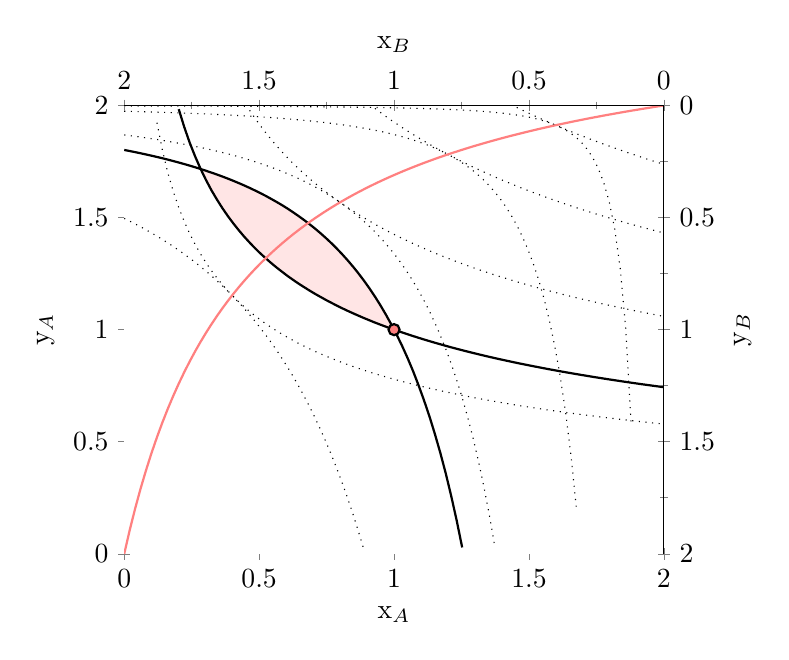
\begin{tikzpicture}[scale=1,thick]
    \def\alpha{0.7}
    \def\beta{0.3}
    \def\L{2}
    \def\K{2}
    \def\PK{0.5}
    \def\PL{0.5}

    \def\InitYA{((\PL*\L)^(1-\alpha))*((\PK*\K)^(\alpha))}
    \def\InitYB{(((1-\PL)*\L)^(1-\beta))*(((1-\PK)*\K)^(\beta))}

    \def\La{0.2*\L}
    \def\Lb{0.4*\L}
    \def\Lc{0.6*\L}
    \def\Ld{0.8*\L}

    \def\Ka{
      \alpha*(1-\beta)*\K*\La/((1-\alpha)*\beta*(\L-\La)+\alpha*(1-\beta)*\La)}
    \def\Kb{
      \alpha*(1-\beta)*\K*\Lb/((1-\alpha)*\beta*(\L-\Lb)+\alpha*(1-\beta)*\Lb)}
    \def\Kc{
      \alpha*(1-\beta)*\K*\Lc/((1-\alpha)*\beta*(\L-\Lc)+\alpha*(1-\beta)*\Lc)}
    \def\Kd{
      \alpha*(1-\beta)*\K*\Ld/((1-\alpha)*\beta*(\L-\Ld)+\alpha*(1-\beta)*\Ld)}

    \def\YAa{((\La)^(1-\alpha)*((\Ka)^\alpha)}
    \def\YAb{((\Lb)^(1-\alpha)*((\Kb)^\alpha)}
    \def\YAc{((\Lc)^(1-\alpha)*((\Kc)^\alpha)}
    \def\YAd{((\Ld)^(1-\alpha)*((\Kd)^\alpha)}

    \def\YBa{((\L-\La)^(1-\beta)*((\K-\Ka)^\beta)}
    \def\YBb{((\L-\Lb)^(1-\beta)*((\K-\Kb)^\beta)}
    \def\YBc{((\L-\Lc)^(1-\beta)*((\K-\Kc)^\beta)}
    \def\YBd{((\L-\Ld)^(1-\beta)*((\K-\Kd)^\beta)}

    \begin{axis}[
        restrict y to domain=0:\K,
        samples = 100,
        xmin = 0, xmax = \L,
        ymin = 0, ymax = \K,
        xlabel = $\mathrm{x}_A$,
        ylabel = $\mathrm{y}_A$,
        axis y line = left,
        axis x line = bottom,
        y axis line style = {-},
        x axis line style = {-}
      ]
      \def\LineA{(\InitYA/\x^(1-\alpha))^(1/\alpha))};
      \def\LineB {\K-(\InitYB/(\L-\x)^(1-\beta))^(1/\beta)};

      \addplot [fill=red!20, opacity=0.5, draw=none,domain=0:\L] {\LineB}
      \closedcycle;
      \addplot [fill=white, draw=none,domain=0:\L] {\LineA} |- (axis cs:0,0)
      -- (axis cs:0,\K)--cycle;

      \addplot[thin, dotted, mark=none, domain=0:\L]
      {(\YAa/\x^(1-\alpha))^(1/\alpha)};
      \addplot[thin, dotted, mark=none, domain=0:\L]
      {(\YAb/\x^(1-\alpha))^(1/\alpha)};
      \addplot[thick, mark=none, domain=0:\L] {(\LineA};
      \addplot[thin, dotted, mark=none, domain=0:\L]
      {(\YAc/\x^(1-\alpha))^(1/\alpha)};
      \addplot[thin, dotted, mark=none, domain=0:\L]
      {(\YAd/\x^(1-\alpha))^(1/\alpha)};

      \addplot[thin, dotted, mark=none, domain=0:\L]
      {\K-(\YBa/(\L-\x)^(1-\beta))^(1/\beta)};
      \addplot[thin, dotted, mark=none, domain=0:\L]
      {\K-(\YBb/(\L-\x)^(1-\beta))^(1/\beta)};
      \addplot[thick, mark=none, domain=0:\L] {\LineB};
      \addplot[thin, dotted, mark=none, domain=0:\L]
      {\K-(\YBc/(\L-\x)^(1-\beta))^(1/\beta)};
      \addplot[thin, dotted, mark=none, domain=0:\L]
      {\K-(\YBd/(\L-\x)^(1-\beta))^(1/\beta)};

      \addplot[mark=none, domain=0:\L, color=red!50,thick]
      {\alpha*(1-\beta)*\K*\x/((1-\alpha)*\beta*(\L-\x)+\alpha*(1-\beta)*\x)};
      \addplot[thick, mark=*, fill=red!50] coordinates {(\L*\PL,\K*\PK)};
    \end{axis}

    \begin{axis}[
        restrict y to domain = 0:\K,
        minor tick num = 1,
        xlabel = $\mathrm{x}_B$,
        ylabel = $\mathrm{y}_B$,
        xmin = 0, xmax = \L,
        ymin = 0, ymax = \K,
        axis y line = right,
        axis x line = top,
        x dir = reverse,
        y dir = reverse,
        y axis line style = {-},
        x axis line style = {-}
      ]
    \end{axis}
  \end{tikzpicture}

  \subsubsection*{General Case}

  \begin{equation*}
    \begin{aligned}
      \max_{\{ (x_{1, 1}, \ldots, x_{1, n}), \ldots, (x_{m, 1}, \ldots, x_{m, n})  \}}\  & u_1 (x_{1, 1}, \ldots, x_{1, n}) \quad         \\
      \text{subject to} \quad                                                            & u_2 (x_{2, 1}, \ldots, x_{2, n}) \ge \bar{u}_2, \\
                                                                                         & \quad \vdots                                   \\
                                                                                         & u_m (x_{m, 1}, \ldots, x_{m, n}) \ge \bar{u}_m; \\
                                                                                         & \sum_{i \in \mathcal{I}} x_{i, 1} \le w_1 ,         \\
                                                                                         & \quad \vdots                                   \\
                                                                                         & \sum_{i \in \mathcal{I}} x_{i, n} \le w_n.
    \end{aligned}
  \end{equation*}

  \begin{boxtheo}
    Let all utility functions be strictly increasing and quasi-concave, and	$((\hat{x}_{1,1}, \ldots, \hat{x}_{1, n}), \ldots, (\hat{x}_{m, 1}, \ldots, \hat{x}_{m, n}))$ be a feasible interior allocation. Then $((\hat{x}_{1,1}, \ldots, \hat{x}_{1, n}), \ldots, (\hat{x}_{m, 1}, \ldots, \hat{x}_{m, n}))$ is \textbf{Pareto-efficient} if and only if $((\hat{x}_{1,1}, \ldots, \hat{x}_{1, n}), \ldots, (\hat{x}_{m, 1}, \ldots, \hat{x}_{m, n}))$ exhausts all resources and, for all pairs of goods $(\ell,\ell')$:
    \[
      \MRS(\ell, \ell') (\hat{x}_{1,1}, \ldots, \hat{x}_{1, n}) = \cdots = \MRS(\ell, \ell') (\hat{x}_{m,1}, \ldots, \hat{x}_{m, n})
      .\]
  \end{boxtheo}

  \newpage

  \subsection{Competitive Equilibrium}

  \subsubsection*{Initial Assumptions}

  \begin{bulletlist}
    \item There is a market for each good.
    \item Every agent can access the market without any cost.
    \item There is a single price for each good.
    \item All consumers know the price.
    \item Each consumer can sell her initial endowment in the market and use the income to buy goods and services.
    \item Consumers seek to maximize their utility given their budget restriction, independently of what everyone else is doing.
    \item There is no centralized mechanism.
    \item People may not know others' preferences or endowments.
    \item There is perfect competition (namely, everyone is a price-taker).
    \item Prices are the only source of information of agents.
  \end{bulletlist}

  \begin{boxdef}[Competitive Equilibrium]
    An ordered pair of an allocation and a price vector, $(X^*, \mathrm{p} = (p_1, \ldots, p_n))$, is called a \textbf{competitive equilibrium} if the following conditions hold:
    \begin{eqlist}
      \item $\forall i \in \mathcal{I},\ \mathrm{x}^*_i = (x^*_{i, 1}, \ldots, x^*_{i, n})$ solves the following maximization problem:
      \begin{equation*}
        \begin{aligned}
          \max_{\{\mathrm{x}_i\}}\quad        & u_i(\mathrm{x}_i)                                                                             \\
          \text{\normalfont subject to} \quad & wh + \left\langle \mathrm{p},\mathrm{x}_i \right\rangle \le \left\langle\mathrm{p},\mathrm{w}_i\right\rangle = \sum_{\ell \in \mathcal{L}} p_\ell w_{i, \ell}.
        \end{aligned}
      \end{equation*}
      \item Markets clear, i.e. $\displaystyle \sum_{i \in \mathcal{I}} x^*_{i, \ell} = \sum_{i \in \mathcal{I}} w_{i, \ell},\ \forall \ell \in \mathcal{L}$.
    \end{eqlist}
  \end{boxdef}

  \begin{boxprop}
    Given, at least, one consumer with strictly monotone preferences. Then, if $(X^*, \mathrm{p})$ is a competitive equilibrium, $p_1, p_2, \ldots, p_n > 0$.
  \end{boxprop}

  \begin{boxprop}
    Given, at least, one consumer with weakly monotone preferences. Then, if $(X^*, \mathrm{p})$ is a competitive equilibrium, for at least one $\ell$, $p_\ell > 0$.
  \end{boxprop}

  \begin{boxprop}
    Let $(X^*, \mathrm{p})$ be a competitive equilibrium. Then, $(X^*, c\mathrm{p})$ is also a competitive equilibrium, $\forall c \in \mathbb{R}_+$.
  \end{boxprop}

  \begin{boxtheo}[Walras' Law]
    If the consumer $i$ has weakly monotone preferences and also $\hat{\mathrm{x}}_i \in \mathrm{x}^*_i (\mathrm{p})$, then:
    \[
      \left\langle\mathrm{p},\hat{\mathrm{x}}_i\right\rangle = \sum_{\ell \in \mathcal{L}} \mathrm{p}_\ell \hat{x}_{i, \ell} = \sum_{\ell \in \mathcal{L}} \mathrm{p}_\ell w_{i, \ell} = \left\langle\mathrm{p},\mathrm{w}_i\right\rangle
      .\]
  \end{boxtheo}

  \begin{boxcor}[Walras' Law]
    Given weakly monotonic utility functions and $\mathrm{p} = (p_1, \ldots, p_n)$ such that $p_\ell > 0$. If any $(X^*,\mathrm{p})$ in which maximization condition holds, $\forall i \in \mathcal{I}$, and markets clear $\forall \ell = 1, 2, \ldots, n - 1$; then, the market clearing condition holds for commodity $n$ as well.
  \end{boxcor}

  \begin{boxtheo}[Fixed Point]
    For any continuous function $f : \triangle^{n - 1} \to \triangle^{n - 1}$, there exists a point $\mathrm{p}^* = (p^*_1, p^*_2, \ldots, p^*_n)$ such that $f(\mathrm{p}^*) = \mathrm{p}^*$, where: $$\displaystyle \triangle^{n - 1} = \left\{(p_1, p_2, \ldots, p_n) \in \mathbb{R}_+^\mathcal{L} : \sum_{\ell \in \mathcal{L}} p_\ell = 1 \right\}.$$
  \end{boxtheo}

  \begin{boxdef}[Shortage]
    We define \textbf{shortage} or \textbf{excess demand} as follows:
    \[
      Z(\mathrm{p}) = (z_1(p), z_2(p), \ldots, z_n(p)) = \sum_{i \in \mathcal{I}} \mathrm{x}^*_i(\mathrm{p}) - \sum_{i \in \mathcal{I}} \mathrm{w}_i
      .\]
  \end{boxdef}

  \begin{boxprop}
    $\mathrm{p}$ is a competitive equilibrium if and only if $Z(\mathrm{p}) = 0$.
  \end{boxprop}

  \sectionbreak

  \subsubsection*{Excess Demand Properties}

  \begin{eqlist}
    \item Continuous in $\mathrm{p}$.
    \item Homogeneous of degree zero.
    \item $\left\langle \mathrm{p},Z(\mathrm{p}) \right\rangle = 0$.
  \end{eqlist}

  \begin{boxprop}
    The equilibrium is not unique.
  \end{boxprop}

  \begin{boxtheo}[Welfare I]
    Given any pure exchange economy such that all consumers have weakly monotonic utility functions. If $(X^*,\mathrm{p})$ is a competitive equilibrium, then $X^*$ is a Pareto-efficient allocation.
  \end{boxtheo}

  \begin{boxtheo}[Welfare II]
    Given an economy $\displaystyle \mathcal{E} = \left\langle \mathcal{I}, (u_i, w_i)_{i \in \mathcal{I}} \right\rangle$ where all consumers have weakly monotonic quasi-concave utility functions. \par
    If $(x_1, x_2, \ldots, x_m)$ is a Pareto-optimal allocation; then, there exists a redistribution of resources $(\hat{w}_1, \hat{w}_2, \ldots, \hat{w}_m)$ and some prices $p = (p_1, p_2, \ldots, p_n)$ such that:
    \begin{eqlist}
      \item $\displaystyle \sum_{i \in \mathcal{I}} \hat{w}_i = \sum_{i \in \mathcal{I}} w_i$.
      \item $(p, (x_1, x_2, \ldots, x_m))$ is a competitive equilibrium of the economy $\mathcal{E}$.
    \end{eqlist}
  \end{boxtheo}

  \newpage

  \subsection{Production}

  \subsubsection*{Initial Assumptions}

  \begin{bulletlist}
    \item There are $k$ firms such that $\mathcal{J} = \left\{ 1, \dots, k \right\}$
    \item The production of firm $j$ for good $l$ is described by the function $f_{j,l}$ such that $f_{j} (\mathrm{z}_{\ell,l}) = f_{j} (z_{1,l}, \dots, z_{n,l})$. Namely, the firm $j$ uses $\mathrm{z}_{\ell}$ units of commodities $\ell \in \mathcal{L}$ to produce commodity $l$.
    \item The firms are owned by consumers in society.
    \item The firms' ownership is exogenous.
    \item $\theta_{ij}$ represents the \emph{fraction} of the firm $j$ owned by the consumer $i$.
    \item The firms do not have endowments.
  \end{bulletlist}

  \begin{boxrmk}
    \[\sum_{i \in \mathcal{I}} \theta_{ij} = \theta_{1j} + \theta_{2j} + \cdots + \theta_{mj} = 1.\]
  \end{boxrmk}

  \begin{boxdef}[Competitive equilibrium]
    $\left( (X^*,Z^*),\mathrm{p} \right)$ is called a \textbf{competitive equilibrium} if the following conditions hold:
    \begin{eqlist}
      \item $\forall j \in \mathcal{J},\ \mathrm{z}^*_j = ((z_{j,1,1'},\dots,z_{j,1,n'}),\dots,(z_{j,n,1'},\dots,z_{j,n,n'}))$ solves the following maximization problem: 
      \[\pi^*_j \quad \deq \quad \max_{\left\{ \mathrm{z}_j \right\}} \quad p_l f_{j,l}(\mathrm{z}_\ell) - \sum_{\ell\in\mathcal{L}} p_\ell \mathrm{z}_{j,\ell}.\]
      \item $\forall i \in \mathcal{I},\ \mathrm{x}^*_i = (x^*_{i,1}, \dots, x^*_{i,n})$ solves the following maximization problem:
      \begin{equation*}
        \begin{aligned}
          \max_{\{\mathrm{x}_i\}}\quad        & u_i(\mathrm{x}_i)                                                                             \\
          \text{\normalfont subject to} \quad & \left\langle \mathrm{p},\mathrm{x}_i \right\rangle \le \left\langle\mathrm{p},\mathrm{w}_i\right\rangle + \sum_{j \in \mathcal{J}} \theta_{ij} \pi^*_j.
        \end{aligned}
      \end{equation*}
      \item Markets clear, namely:
      \[\sum_{i \in \mathcal{I}} x^*_{i,\ell} + \sum_{j \in \mathcal{J}} \sum_{\ell \in \mathcal{L}} \mathrm{z}^*_{j,\ell} = \sum_{i \in \mathcal{I}} w_{i,\ell} + \sum_{j \in \mathcal{J}} f_{j,l} (\mathrm{z}^*_\ell) .\]
    \end{eqlist}
  \end{boxdef}

  \begin{boxprop}
    Walras' law and welfare theorems hold.
  \end{boxprop}

  \begin{boxprop}
    Let $((X^*,Z^*),\mathrm{p})$ be a competitive equilibrium. \par Then, $((X^*,Z^*), c\mathrm{p})$ is also a competitive equilibrium, $\forall c \in \mathbb{R}_+$.
  \end{boxprop}

  \emph{Note:} with production, Edgeworth box illustrations are no longer helpful.

  \subsubsection*{General Case}

  \begin{equation*}
    \begin{aligned}
      \max_{\{X,Z\}} \quad    & u_1(\mathrm{x}_1) \\
      \text{subject to} \quad & u_2(\mathrm{x}_2) \geq \bar{u}_2, \\
                              & \quad \vdots \\
                              & u_m(\mathrm{x}_m) \geq \bar{u}_m; \\
                              & \sum_{i \in \mathcal{I}} x_{i,1} + \sum_{j \in \mathcal{J}} z_{j,1} \leq \sum_{j \in \mathcal{J}} f_{j,1} (\mathrm{z}_\ell) + \sum_{i \in \mathcal{I}} w_{i,1}, \\
                              & \quad \vdots \\
                              & \sum_{i \in \mathcal{I}} x_{i,n} + \sum_{j \in \mathcal{J}} z_{j,n} \leq \sum_{j \in \mathcal{J}} f_{j,n} (\mathrm{z}_\ell) + \sum_{i \in \mathcal{I}} w_{i,n}.
    \end{aligned}
  \end{equation*}

  \begin{boxtheo}
    Let all utility functions be strictly increasing and quasi-concave, and $(\hat{X},\hat{Z})$ be a feasible interior allocation. Then, $(\hat{X},\hat{Z})$ is \textbf{Pareto-efficient} if and only if all of the following equalities hold for all pairs of goods $(\ell,\ell')$:
    \begin{eqlist}
      \item Marginal rates of substitution are equal across consumers for any pair of commodities, \[\ie \quad \MRS(\ell,\ell')(\hat{\mathrm{x}}_1) = \cdots = \MRS(\ell,\ell')(\hat{\mathrm{x}}_m).\]
      \item Marginal rates of technical substitution are equal across firms for any pair of commodities, \[\ie \quad \MRTS(\ell,\ell')(\hat{\mathrm{z}}_1) = \cdots = \MRTS(\ell,\ell')(\hat{\mathrm{z}}_k).\]
      \item Marginal rates of transformation are equal to the marginal rates of substitution, \[\ie \quad \MRT(j,j')(\hat{\mathrm{z}}_{\ell''}) = \MRS(\ell,\ell')(\hat{\mathrm{x}}_i), \quad \forall i \in \mathcal{I}.\]
    \end{eqlist}
  \end{boxtheo}

  \begin{boxdef}[Production possibility set]
    We define the \textbf{production possibility set} as the set of all non-negative outputs of goods that the firms can produce using the economy's available factor inputs. The output combinations on the \emph{frontier} of this set correspond to the \emph{Pareto-efficient allocation} of factor inputs, i.e. the allocation in which it is not possible, given the total factor endowment, to increase the production of one good without decreasing the production of some other good.
  \end{boxdef}

  \sectionbreak

  \begin{boxrmk}[A friendly reminder on marginal rates]
    \textbf{Marginal rate of substitution (MRS)}
    \begin{bulletlist}
      \item It is the rate at which a consumer is willing to trade one good for another to maintain a constant level of utility.
      \item It is the slope of an \emph{indifference curve}.
      \item It focuses on demand side of consumer theory.
    \end{bulletlist}
    \textbf{Marginal rate of transformation (MRT)}
    \begin{bulletlist}
      \item It is the amount of one good that must be given up to produce an additional unit of another good.
      \item It is the slope of \emph{production possibility frontier}.
      \item It focuses on supply side of a commodity.
    \end{bulletlist}
    \textbf{Marginal rate of technical substitution (MRTS)}
    \begin{bulletlist}
      \item It is the amount by which the quantity of one input has to be reduced in order to use another input.
      \item It is the slope of an \emph{isoquant curve}.
      \item It focuses on production side of economic theory.
    \end{bulletlist}
  \end{boxrmk}

  \newpage

  \section{Monopoly and Monopsony}

  \begin{boxdef}[Monopoly]
    A \textbf{monopoly} is a single supplier of a market. This firm may choose to produce at any point on the market demand curve. For such reason, there is \emph{no monopoly supply curve}.
  \end{boxdef}

  \begin{boxrmk}[Price-taking]
    We say that a firm has a \emph{price-taking} behavior if it cannot dictate prices in the market.
  \end{boxrmk}

  \subsubsection*{Firms' problem}

  \[\max_{\left\{ x \right\}} \quad p(x)x - c(x),\]

  or

  \[\max_{\left\{ p \right\}} \quad pq(p) - c(q(p));\]

  where $p(x)$ is the \textbf{demand} function and $q(p)$ is the \textbf{inverse demand} function.

  \begin{boxdef}[Revenue]
    We define the \textbf{revenue} of the firm as follows:
    \[R(q) = p(q)q.\]
  \end{boxdef}

  \begin{boxprop}
    \[\frac{dR}{dq} = p(q) + q \frac{dp}{dq}(q) = p(q) \left( 1 + \frac{1}{\E_{q,p}} \right).\]
    \emph{Note:} $\E_{q,p}$ is the elasticity of demand with respect to price.
  \end{boxprop}

  \begin{boxprop}
    We say that the demand is \emph{inelastic} if $\E_{q,p} \in (-1,0)$, thus:
    \begin{bulletlist}
      \item An increase in price leads to a small decrease in demand.
      \item An increase in quantity leads to a big decrease in price.
    \end{bulletlist}
    Likewise, we say that the demand is \emph{elastic} if $\E_{q,p} < -1$, thus:
    \begin{bulletlist}
      \item An increase in price leads to a big decrease in demand.
      \item An increase in quantity leads to a small decrease in price.
    \end{bulletlist}
  \end{boxprop}

  \begin{boxprop}
    Whenever the demand function has constant elasticity $\kappa$, namely: $\E_{q,p} = \kappa < 0$. Then:
    \[q(p) = Ap^\kappa \iff p(q) = \left( \frac{q}{A} \right)^{\nicefrac{1}{\kappa}}, \quad \forall A = e^C > 0.\]
  \end{boxprop}

  \begin{boxrmk}
    A monopoly firm always produces at a point such that demand is \emph{elastic}. Which lead us to:
    \[p = \frac{1}{1 + \left(\displaystyle \nicefrac{1}{\E_{q,p}}\right)} \frac{dc}{dq} > \frac{dc}{dq}.\]
  \end{boxrmk}

  \begin{boxrmk}
    The quantity produced $q$ is below the quantity where $\displaystyle p = \frac{dc}{dq}$.
  \end{boxrmk}

  \begin{boxprop}
    Whenever the demand function has constant elasticity $\kappa \geq -1$, the firm will always prefer to increase the price and there is no solution.
  \end{boxprop}

  \subsection{Price discrimination}

  \begin{boxdef}[Price discrimination]
    A monopoly engages in \textbf{price discrimination} if it is able to sell otherwise identical units of output at different prices.
  \end{boxdef}

  \begin{boxdef}[First-degree price discrimination]
    \textbf{First-degree price discrimination} occurs when each buyer can be separately identified by a monopolist, then it may be possible to charge each maximum price they would willingly pay for the good. Namely, this strategy would then extract all available consumer surplus, leaving demanders as a group indefferent between buying the monopolist's good or doing without it. This is also called \textbf{perfect price discrimination} or \textbf{one-to-one marketing}.
  \end{boxdef}

  \begin{boxprop}
    Given a monopoly with a \textbf{perfect price discrimination} strategy, all the followin conditions hold:
    \begin{bulletlist}
      \item Consumer surplus equals zero.
      \item The firm will price at $p(q)$ for the $q$-th unit and continue to produce until $p(q^*) = c'(q^*)$.
      \item The firm's profit is: \[\pi = \int_{0}^{q^*} p(q)dq - c(q^*).\]
      \item There is no deadweight loss.
    \end{bulletlist}
  \end{boxprop}

  % \begin{boxdef}[Second-degree price discrimination]
  %   A
  % \end{boxdef}

  % \begin{boxdef}[Third-degree price discrimination]
  %   A
  % \end{boxdef}

  \newpage

  \section{Game Theory}

  \vfill\eject
  \columnbreak
\end{multicols}
\end{document}
